\documentclass{article}

\usepackage{titlesec}
\usepackage{titling}
\usepackage[margin=0.9in]{geometry}
\usepackage[backend=bibtex, style=authoryear, natbib]{biblatex}
\usepackage{graphicx}
\usepackage{wrapfig}
\usepackage{booktabs}
\usepackage{standalone}
\newcommand{\tabitem}{~~\llap{\textbullet}~~}
\setlength\intextsep{0pt}

\bibliography{computing_references}

%Code
\usepackage{listings}                                                                                                                     
\usepackage{color}

\definecolor{dkgreen}{rgb}{0,0.6,0}
\definecolor{gray}{rgb}{0.5,0.5,0.5}
\definecolor{mauve}{rgb}{0.58,0,0.82}

\lstset{frame=tb,
  aboveskip=3mm,
  belowskip=3mm,
  showstringspaces=false,
  columns=flexible,
  basicstyle={\small\ttfamily},
  numbers=left,
  numberstyle=\tiny\color{gray},
  keywordstyle=\color{blue},
  commentstyle=\color{dkgreen},
  stringstyle=\color{mauve},
  breaklines=true,
  breakatwhitespace=true,
  tabsize=3
}
%Title formatting
\titleformat{\section}{\Large\bf}{}{0em}{}[\titlerule]

\title{CT4021 Introduction To Programming Fundamentals\\\large Assignment 2 - A Personalized Home Security System}
\author{Sam Slade}
\date{}

\begin{document}
\maketitle

\section*{Introduction}
  \documentclass{article}
\begin{document}
  The product developed in this project is a home security system.
  It allows for the locking of a door with a servo motor, which can be opened with use of a key code.
  The key code can be entered on the security systems keypad.
  A small LCD is used to display messages indicating the current state of the security system, i.e. is the door locked or unlocked.
  Further feedback is given to the user by a small piezoelectric speaker and different coloured LEDs.
  These are used to communicate when buttons on the keypad are pressed and when the door is locked and unlocked.
  The most important component of the entire project is the Arduino Uno board, it's the brains of the entire operation and controls the input and output of every other component used.
  The use of the Arduino also allows for multiple codes to be stored and for the codes to be edited all without the need for rebooting or reflashing of memory.

  During the development of the project a number of challenges were faced, some more difficult than others.
  A recurring issue was the lack of digital input and output pins (which will be referred to as I/O pins from now) on the Arduino Uno board.
  One solution to this problem would have been to move away from the Arduino Uno board to an Arduino Mega which has many more digital I/O pins allowing for the use of more components.
  However, the solution chosen to this issue was to use a 74HC595N shift register, more will be spoken about the shift register in the design section of this report.
  As well as the use of the shift register, wiring choices were carefully considered, by the end of the project the two LEDs used didn't use any of the digital I/O pins but would still light up when appropriate.

  
\end{document}


\section*{Design Of The System}
  \begin{document}
  \subsection*{Hardware}
  
  While developing this project, an agile-like methodology was adopted.
  Each two week sprint ended with a review of what had been done towards the project and what would be done in the next sprint.
  Focus shifted from sprint to sprint but each had to produce something useable towards the final product.
  Keeping track of tasks in each sprint and between sprints was made easier with tools such as Trello which uses the Kanban system for organising tasks.

  In the earlier sprints, the focus was on understanding each of the components that would be used in the final product.
  As well as gaining understanding, the early sprints were also used to produce code blocks that could be utilised in the final code build.
    Later sprints looked at assembling what was learnt into the final circuit.
  Figure \ref{fig:one} shows one of the first designs for the circuit taken from an early sprint, there are a number of issues in this design that will now be discussed before looking at the final design to show the changes that were made throughout the development cycle.
  This initial design shows the LCD, keypad, piezoelectric speaker and LED all wired to the Arduino Uno.
  This design didn't include the servo motor required by the design specification as there weren't enough digital I/O pins to support it.
  Other issues with this design included the use of digital pins zero and one.
  Using pins zero and one can cause an issue where, during the flashing process, the program counter becomes de-synchronised, this is caused by the tiny amount of resistance of the wires being in pins zero and one.
  The wires could be removed each time the Arduino's memory is written to but this later became more difficult as larger numbers of wires were added to the system.
  In a later version, it was decided to remove the use of pins zero and one to completely avoid this issue.
  The initial design also included only one LED, which was okay but to allow for better indication of what state the system is in, there was a need for more LEDs of different colours.
 \begin{figure}[h]
    \vspace{0.3cm}
    \begin{center}
      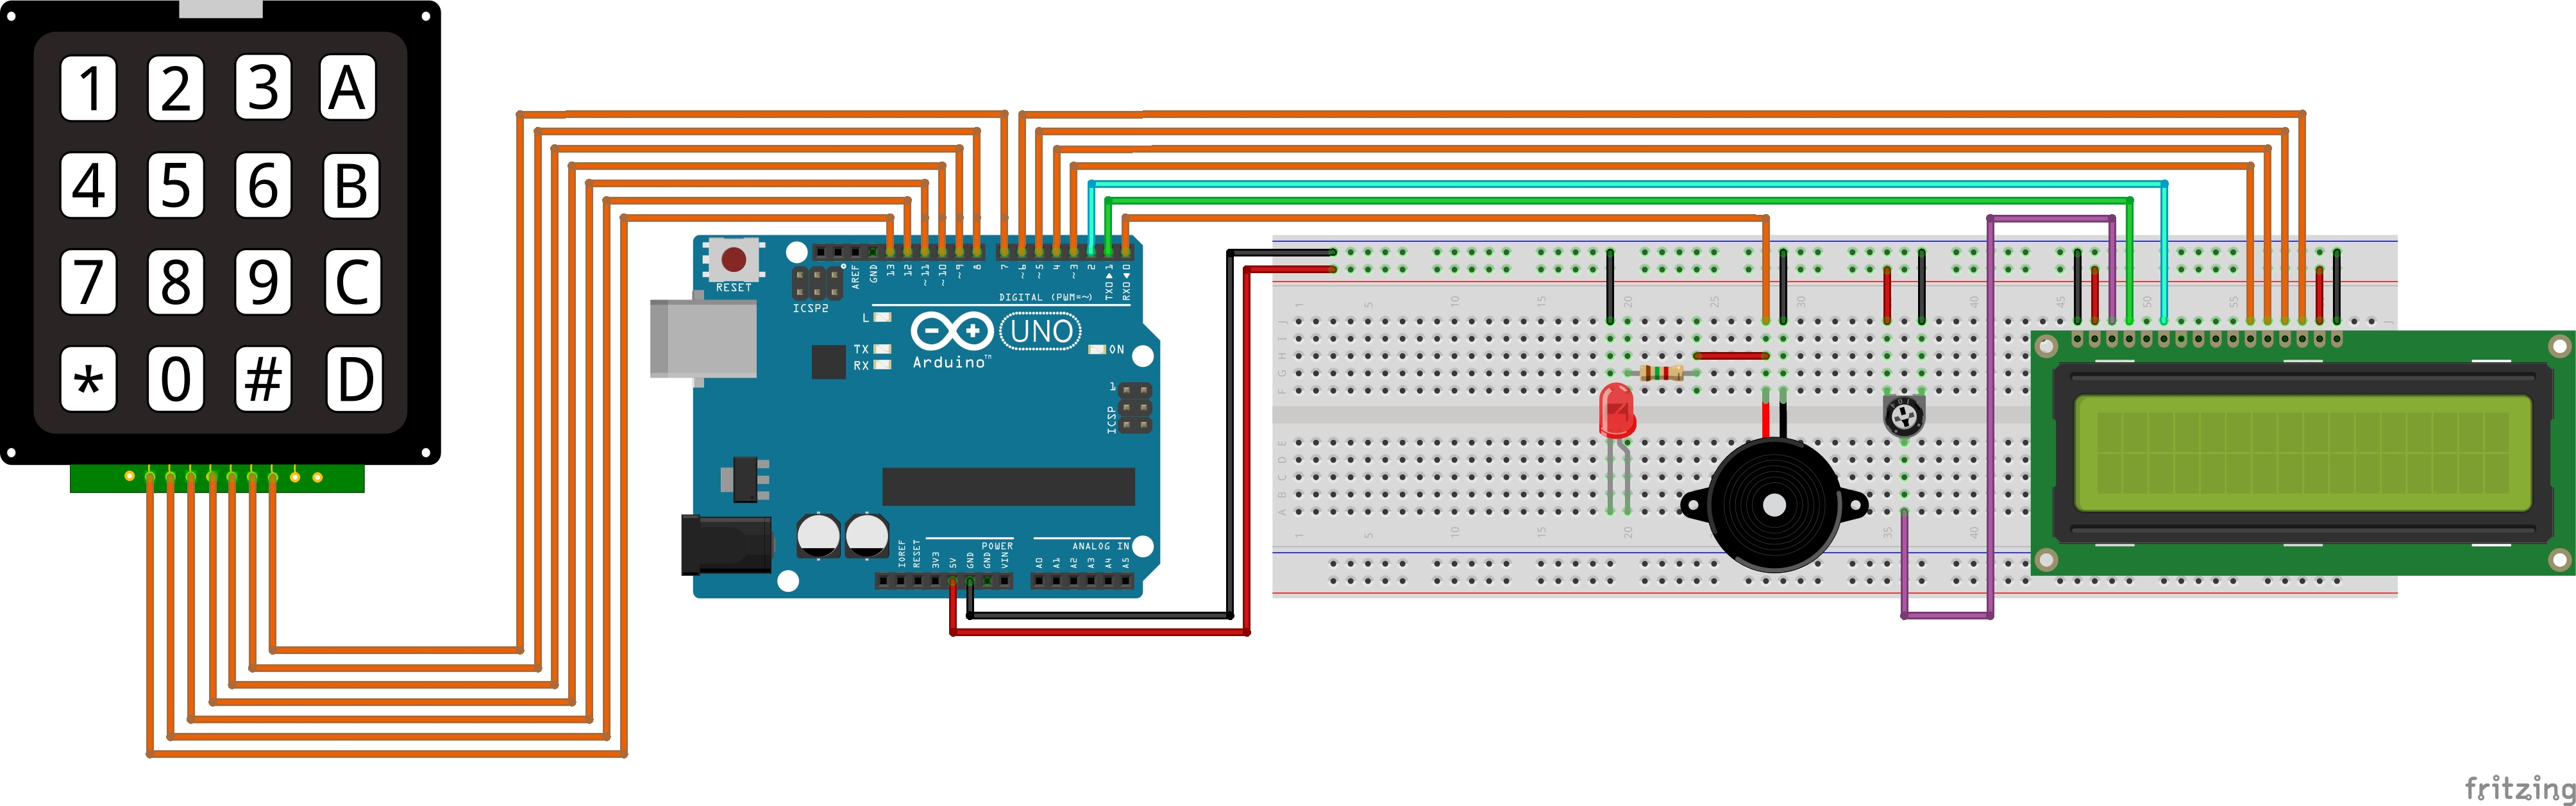
\includegraphics[width=0.68\textwidth]{initial.jpg}
    \end{center}
    \vspace{-20pt}
    \caption{Initial design using Fritzing}
    \label{fig:one}
    \vspace{0.3cm}
  \end{figure}

    The final design reached sought to correct each of these issues, Figure \ref{fig:two} shows the final design.
  The largest change from the initial design is that the LCD is no longer directly connect to the Arduino.
  Instead, the Arduino connects to a 74HC595N shift register which then connects to the LCD.
  lastminuteengineers (no date), sates that the [shift register] essentially controls eight separate output pins, using only three input pins.
  Normally, the LCD requires seven connections to the data pins on the Arduino, using the shift register allows for the LCD to be controlled using only three digital I/O pins.
  This means four more connections can be made to the Arduino while losing no functionality and freeing up digital I/O pins zero and one.
  The digital I/O pins used by the shift register had to be pins nine, eleven and thirteen, as these are the digital I/O pins that provide the Serial Peripheral Interface (SPI).
  SPI is a synchronous serial communication method, which the shift register requires in order to send the data correctly onto the LCD.
  Getting the shift register to work with the LCD also meant using a modified LCD header file provided by Juan Hernandez (Hernandez, 2016). 
    The final design also makes use of multiple LEDs which are connected to the piezoelectric speaker's and the servo motor's digital I/O pin as well.
  This means that by carefully controlling when the piezoelectric speaker is used, the red LED will light up and when the servo motor is used, the green LED will light up.
  An RGB LED was originally planned to be used, but due to a wiring error, the LED was damaged and couldn't be used in the final product.

  As was mentioned in the previous paragraph, the servo motor was also implemented in the final design using the extra digital I/O pins available.
  The servo motor is used to open and close the lock in the door, it is controlled by the Arduino and when the correct code is entered on the key pad, then the servo motor will open.
  The keypad, in both the initial and final design isn't fully connected.
  The right most column (containing the buttons A, B, C and D) is not connected, this is to free more I/O pins to be left available for other components. 
      \begin{figure}[h]
        \vspace{0.3cm}
        \begin{center}
        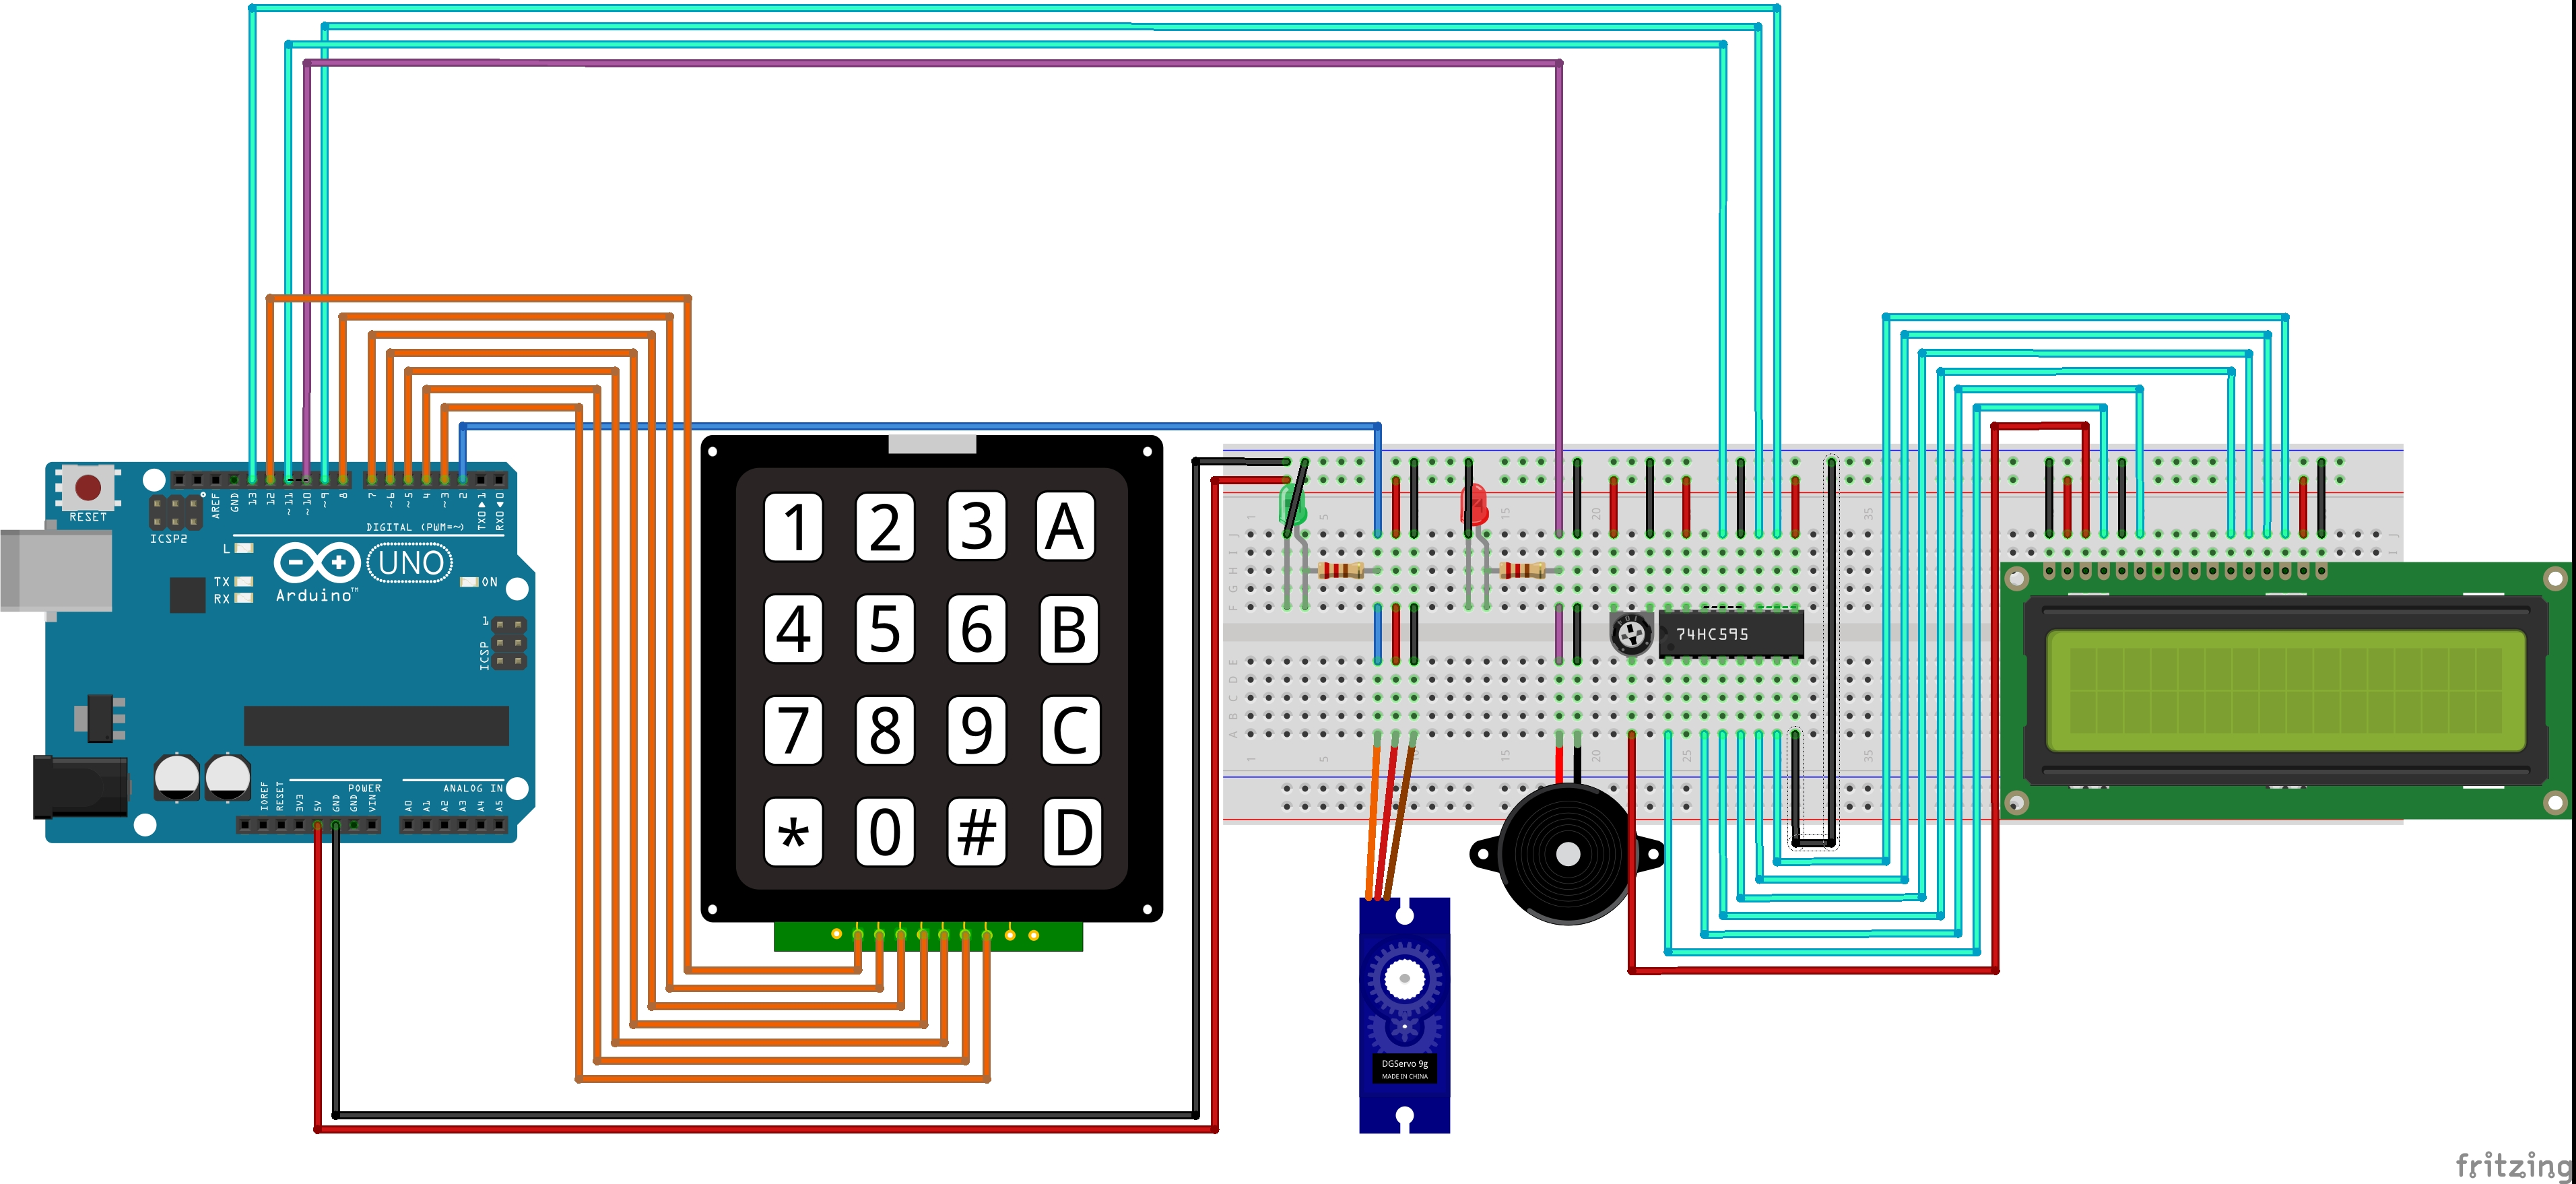
\includegraphics[width=0.68\textwidth]{final.jpg}
        \caption{Final design using Fritzing}
        \label{fig:two}
        \end{center}
        \vspace{0.3cm}
      \end{figure}

  \newpage

  \begin{figure}[h]
    \begin{center}
    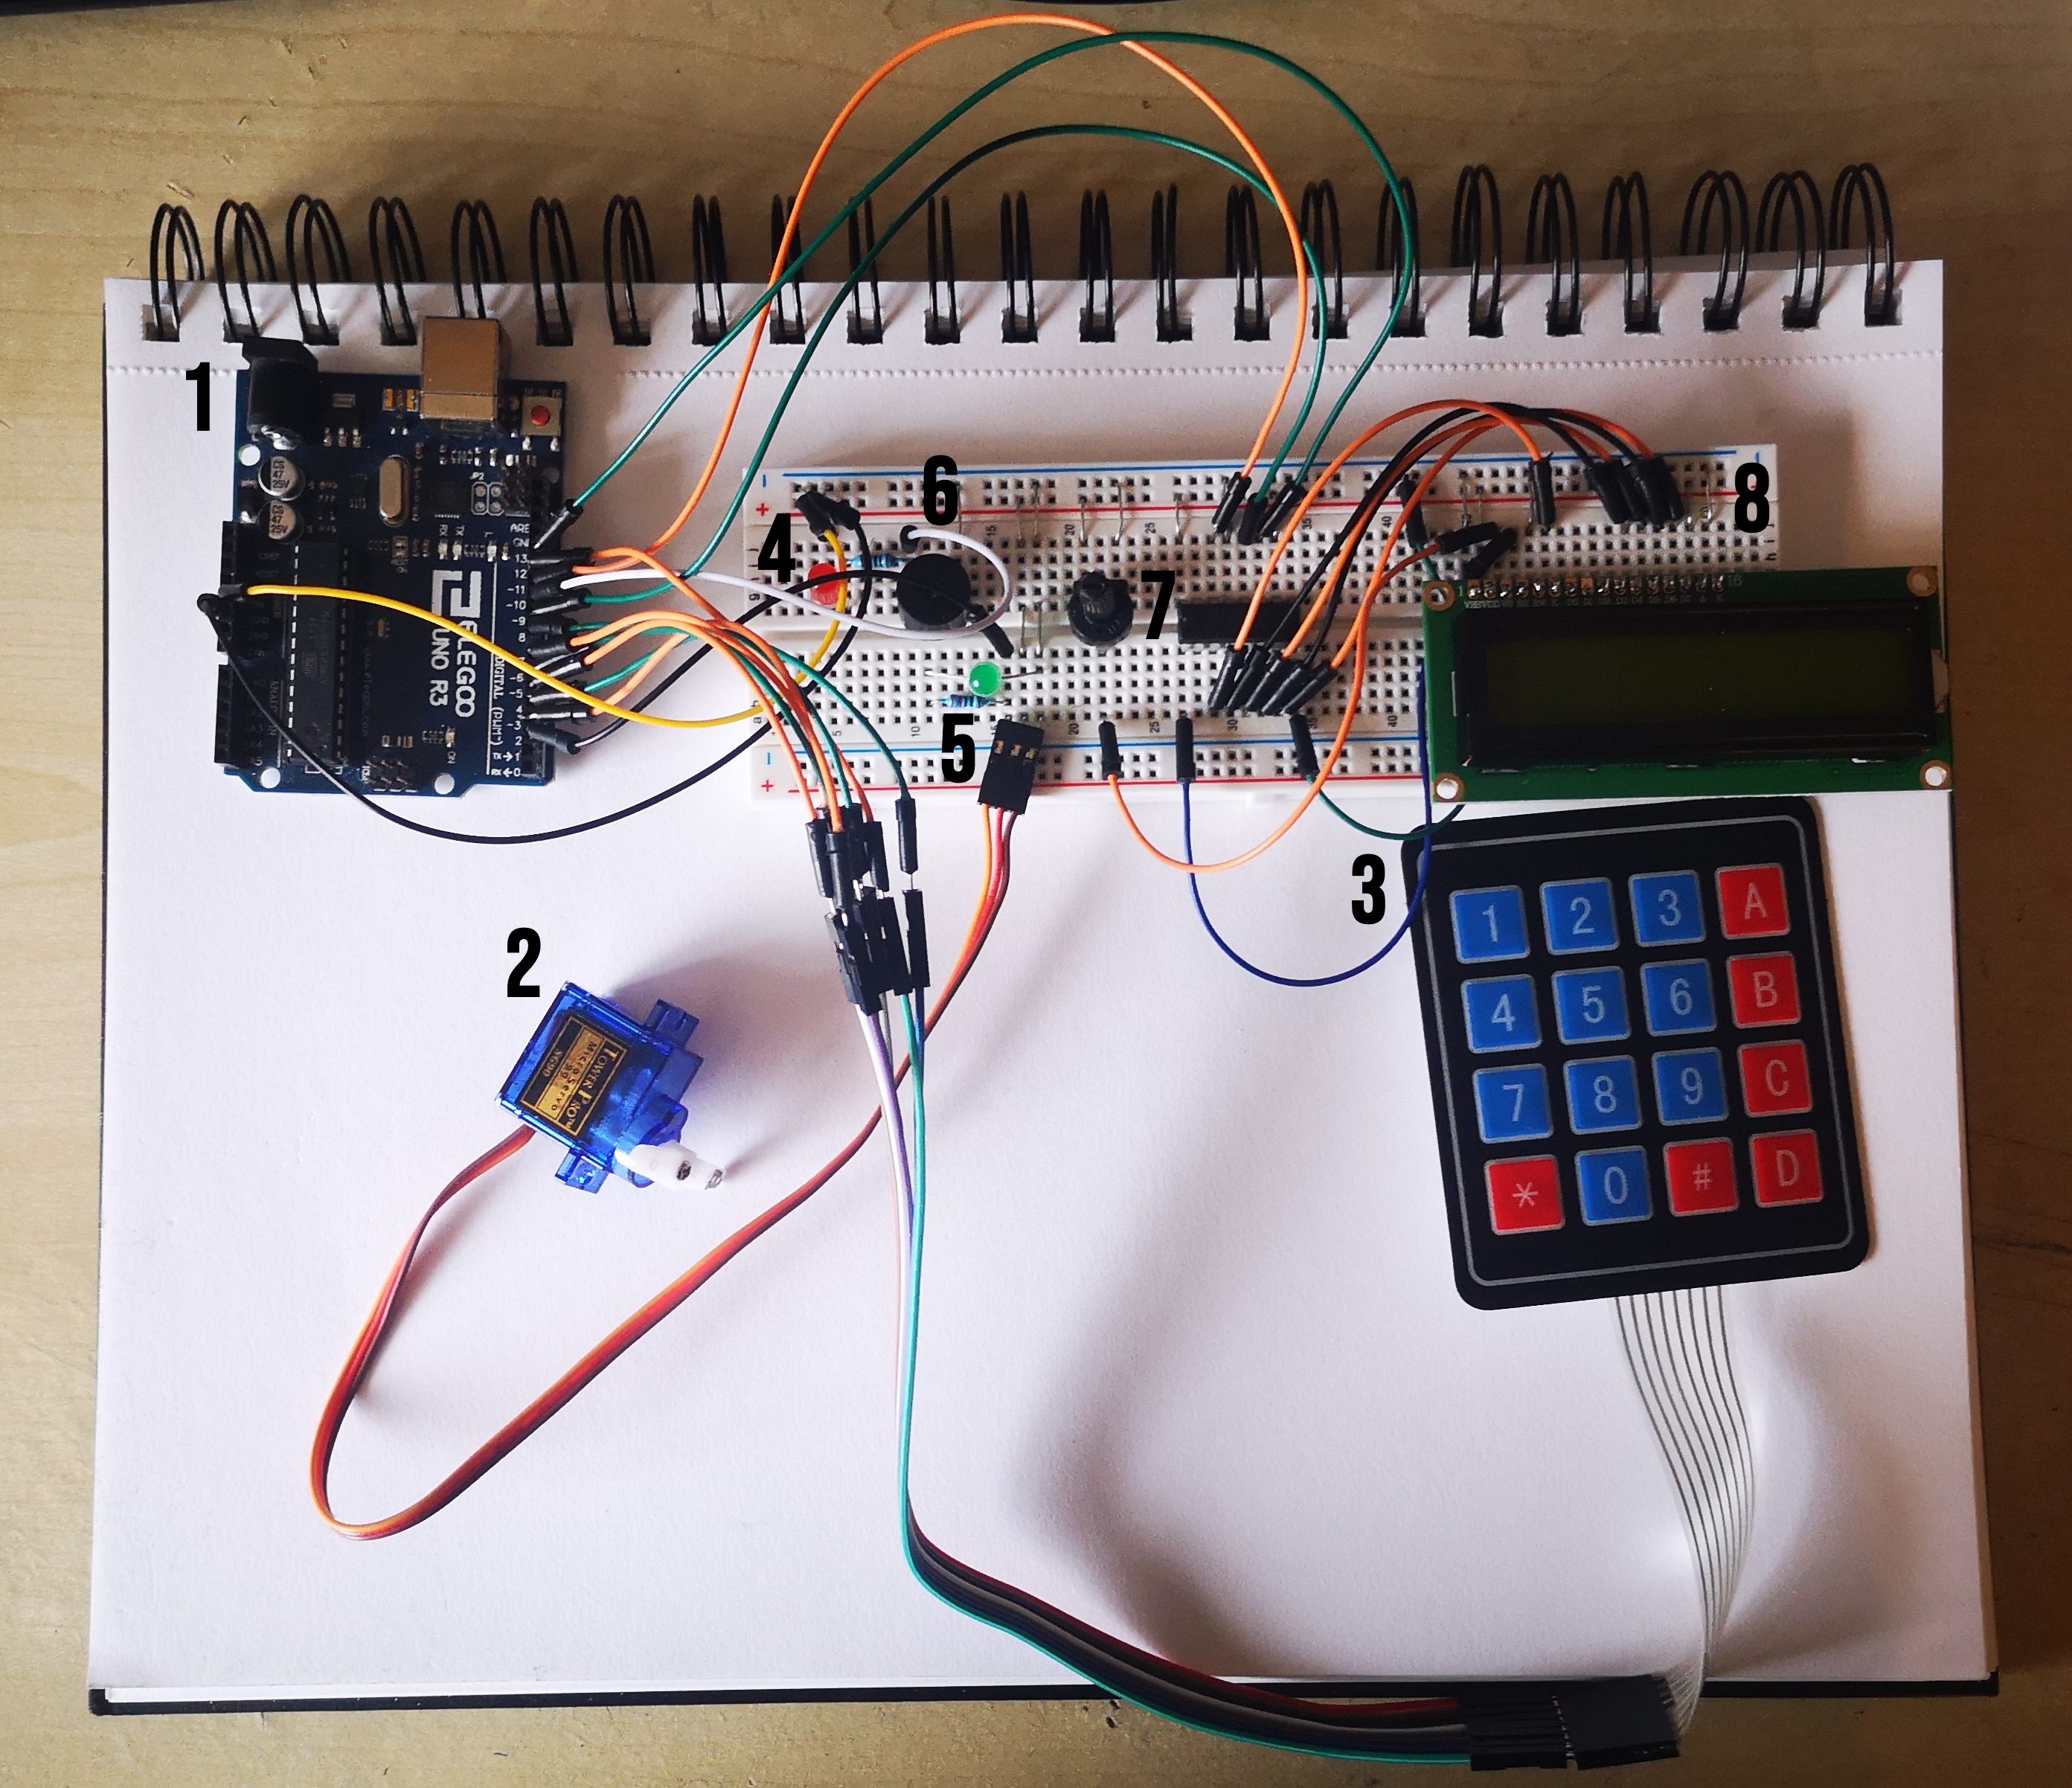
\includegraphics[width=0.8\textwidth]{labelled.jpg}
    \caption{Labelled circuit of the final design}
    \end{center}
  \end{figure}
  \begin{enumerate}
  \item Arduino Uno
  \item Servo Motor
  \item Keypad
  \item Red LED
  \item Green LED
  \item Piezoelectric Speaker
  \item 74HC595 Shift Register
  \item LCD
  \end{enumerate}
  \subsection*{Software}
  When developing the software for the project, it was decided early on to use heap allocated arrays to store the codes entered by the user.
  This choice allowed for better control of when and where memory was allocated and de-allocated, this is important as Guyer and Helbling (2016) note, typically [the Arduino has] 32 KB of flash memory for the program  and  2  KB  of  RAM  for  both  the  stack  and  heap.
  These limitations place significant constraints on how the boards are programmed.

  \lstinputlisting[language=C, firstline=50, lastline=58, caption=Declaring pin code storage variables\\\hspace{\textwidth} (assignment\_code.ino line 50-58), label=lst:one]{assignment_code.ino}

  Listing \ref{lst:one} shows the variable \verb|pinCodeArray| being defined, this is an array of char pointers to other char pointers, often called a multi-dimensional array.
  The array will be used to store the different user codes.
  This method does require more memory with the use of pointers to each array, but it does remove the need for a larger number of named variables, which was considered to be a valuable trade off.
  The variable \verb|input| was also defined here, which is a char pointer that can hold four characters.
  This is used to store the code being entered by the user on the keypad.
  The variable \verb|pointer| is used to keep track of which digit has been entered by the user.
  Listing \ref{lst:two} shows the Arduino \verb|setup| function and how it was used to set the user pin code array.
  Also in the setup function, line 2 is for setting up the serial debugging mode, line 7 is to initialise the LCD with a display size of two lines and 16 characters per line and line 10 is to set up the pin connected to the piezoelectric speaker.
  From line 14, the pin code array is being setup, 14 to 16 is a for loop that gives each of the pin code array elements a pointer to a four character array.
  These four character arrays are the codes used to unlock the system.
  Lines 18 to 23 are a set of nested for loops used to set each of the values in the four character arrays to be \verb|NULL|, this is done to remove the risk of a memory leak.
  Finally, lines 27 to 35 are used to set the admin code which is used to edit the other codes in the system.
  The admin code is set to the value \verb|0, 1, 2, 3| using a for loop and the \verb|itoa| function.
  This function takes three parameters, an integer, a char pointer and a second integer which is used to describe the base of the first integer.
  The function converts the first integer into a string and stores it in the character pointer.
  The value in the character pointer is then stored in the four character array at index zero in the pin code array, this can be seen on line 33.

  \lstinputlisting[language=C, firstline=77, lastline=111, caption=Setting up the code storage array and setting the default admin pass code\\\hspace{\textwidth} (assignment\_code.ino line 77-111), label=lst:two]{assignment_code.ino}

  The largest piece of the source code is taken up by the \verb|admin_menu| function.
  The code snippet for the \verb|admin_menu| function is too large for this section of the document and can be found in Appendix \ref{code} at lines 282 to 429.
  The function allows the user to edit codes on the system and can be accessed by entering the admin code on the keypad.
  To do this, the function first enters a while loop, this is used to keep checking key presses from the user, from here the user can be sent back to the main locked screen or enter the next while loop and choose a code, number 0 through 9, to edit.
  When the user enters a valid number the next while loop is entered, this prompts the user to enter a new code and then repeat the new code.
  The new code and the repeated code are store inside heap allocated arrays, to protect the system from a memory overflow, the two arrays are deallocated on lines 359 and 360.
  Lines 339 to 374 are used to store the new codes that are entered by the user.
  The two codes are first checked to see if they are the same, if not then the user is prompted to enter new codes.
  If the two codes entered are identical then, using a for loop, the new code is copied into the \verb|pinCodeArray| variable, the new code arrays are deallocated and then the function returns.
\end{document}


\section*{Testing The System}
  \begin{document}
  The testing process for the product began with the writing of user stories.
  The user stories can be found in Appendix \ref{user stories}, these detail the criteria that the product should meet to be feature complete.
  From the user stories, a set of unit tests were developed.
  The unit tests can be found in Appendix \ref{test suites}.
The first unit test 001, concerns the admin menu, for this function to succeed the system needs to identify the admin code correctly and then take the users input for the new codes and store them correctly.
This test covers a large portion of the code base, including the feedback functions and the logic inside the \verb|admin_menu| function.
Unit test 002, is then making sure that the user cannot enter an invalid admin code and gain access to the admin menu, this again tests the systems logic to make sure the code is checked properly.
Test 003 and 004 move to check the user codes which open the door but don't allow access to the admin menu.
Test 003, checks to see if a valid code works and so covers code validation as well as checks to see if the servo motor functions properly.
Test 004 then makes sure that an invalid code cannot be used.
Test 005, will have been partially tested by the other unit tests but tests the systems feedback to the user from pressing buttons on the keypad.
These unit tests cover the main cases for using the system and checks nearly the entire code base.
There maybe edge cases which haven't been considered which is why there is hesitance to commit to all of the code being fully checked.
However, each key area of function has been unit tested individually and all have succeeded.
\end{document}

  
\newpage
\section*{Appendix}
  \subsection{Evidence Video}
    https://www.youtube.com/watch?v=eQMCCoCKMT0&t=6s
  \subsection{User Guide}
    \subsubsection{System diagram}
\subsubsection{Unlocking a door using the system}
  To unlock a door using the system, a valid \textit{user code} must be entered.
  A \textit{user code} can be set in the admin menu, details for doing this can be found in section \ref{sec:user_guide_user}.
  The \textit{user code} is entered using the keypad.
  The number of digits the user has entered will be displayed on the LCD.
  When a valid user code is entered, the LCD will display a ``SUCCESS'' message accompanied by the green LED lighting up.
  Finally, the servo motor will move into the unlocked position.
  After a few seconds, the servo motor will return to the locked position.

\subsubsection{Opening and closing the admin menu}\label{sec:user_guide_admin}
  To open the admin menu, the \textit{admin code} must be entered, by default the \textit{admin code} is \verb|0, 1, 2, 3|.
  The \textit{admin code} is entered on the keypad.
  When the valid \textit{admin code} is entered, the admin menu is then displayed on the LCD.\\

  To close the admin menu, simply press 2 on the keypad.

\subsubsection{Changing the default admin code}
  To change the default \textit{admin code}, first navigate to the admin menu, details on how to do this can be found in section \ref{sec:user_guide_admin}.
  After navigating to the admin menu, press 1 on the keypad, this will begin the process of editing a code.
  When prompted to choose the code to edit, press 0 on the key pad to edit the \textit{admin code}.
  Follow the prompts on the LCD by entering the new \textit{admin code}, then re-entering the \textit{admin code}.
  After the \textit{admin code} has been entered and re-entered successfully, you will be taken back to the main screen on the LCD.
  If an invalid code is entered, you will be asked to re-enter the number of the code to edit.

\subsubsection{Adding and changing a user code}\label{sec:user_guide_user}
  To add and change a \textit{user code}, first navigate to the admin menu, details on how to to do this can be found in the section \ref{sec:user_guide_admin}.
  After navigating to the admin menu, press 1 on the keypad, this will begin the process of editing a code.
  When prompted to choose the code to edit, enter a number between 1 and 9 on the keypad to edit or create the \textit{user code} assigned to that number.
  Follow the prompts on the LCD by entering the new \textit{user code}, then re-entering the \textit{user code}.
  After the \textit{user code} has been entered and re-entered successfully, you will be taken back to the main screen on the LCD.
  If an invalid code is entered, you will be asked to re-enter the number of the code to edit.
  



  \subsection{Code} \label{code}
    \begin{document}
\lstinputlisting[language=C,  caption=assignment\_code.ino]{assignment_code.ino}
C, firstline=50, lastline=58, caption=assignment\_code.ino]{assignment_code.ino}
\end{document}


  \subsection{User Stories} \label{user stories}
    \begin{document}
  \begin{center}
    \begin{tabular}{|l|l|}
      \hline
      \textbf{User Story ID} &
      \textbf{User Story Description}\\ 
      \hline

      001 &
      The user can enter a code and open the door \\ 
      \hline

      002 & 
      The user can enter an invalid code and the code will be rejected \\ 
      \hline

      003 & 
      The user can enter an admin code to edit the other codes \\ 
      \hline

      004 & 
      The user can enter a non-admin code and the admin menu will not be opened \\ 
      \hline

      005 &
      The user will get feedback when using the system \\ 
      \hline
    \end{tabular}
  \end{center}
\end{document}


  \subsection{Test Suites} \label{test suites}
    \begin{document}
  \begin{center}
    \begin{tabular}{|p{1cm}|p{1cm}|p{3cm}|p{3cm}|p{3cm}|p{4cm}|}
      \hline
      \textbf{Test Reference No.} & 
      \textbf{User Story ID} &
      \textbf{Description of test} &
      \textbf{Testing Process} & 
      \textbf{Expected outcome} & 
      \textbf{Actual outcome}\\ 
      \hline

      001 & 
      003 &
      The user enters a valid admin code and can edit a code. &
      \begin{itemize}
        \item User enters a valid admin code
        \item User enters number of code to edit
        \item User enters new code
        \item User re-enters the new code
      \end{itemize} &
      The system accepts the new code and will then take the user back to the main ``locked'' screen. &
      This unit test was successful. The system accepted the new code entered by the user and then took the user back to the main ``locked'' screen.\\ \hline

      002 &
      004 &
      The user enters an invalid admin code and will be rejected by the system &
      \begin{itemize}
        \item User enters an invalid admin code
      \end{itemize} &
      The system will reject the code and provide feedback to the user. &
      This unit test was successful. The system rejected the code and provided feedback in the form of flashing the LED and using the piezoelectric speaker.\\ \hline
    \end{tabular}

    \newpage

    \begin{tabular}{|p{1cm}|p{1cm}|p{3cm}|p{3cm}|p{3cm}|p{4cm}|}
      \hline
      \textbf{Test Reference No.} & 
      \textbf{User Story ID} &
      \textbf{Description of test} &
      \textbf{Testing Process} & 
      \textbf{Expected outcome} & 
      \textbf{Actual outcome}\\ 
      \hline

      003 &
      001 &
      The user enters a valid code to open the door using the servo. &
      \begin{itemize}
        \item User performs test 001 to create a valid code
        \item User enters the valid code
      \end{itemize} &
      When the valid code is entered the servo will open and then close. &
      This unit test was successful. Test 001 was done successfully. The code created was then accepted by the system when entered by the user. The servo opened and then closed, accompanied by feedback from the green LED.\\\hline

      004 & 
      002 &
      The user enters an invalid code and the system will reject the code. & 
      \begin{itemize}
        \item User performs test 001 to create a valid code
        \item User enters an invalid code
      \end{itemize} &
      When the user enters the invalid code, the system rejects the code &
      This unit test was successful. Test 001 was done successfully. The invalid code was entered and the system rejected it and gave feedback with the red lED and piezoelectric speaker.\\ \hline

      005 &
      005 &
      The user receives feedback from the system &
      \begin{itemize}
        \item The user presses buttons on the keypad, producing a tone from the piezoelectric speaker
        \item The user performs test 001 and creates a valid code
        \item The user enters the valid code, getting feedback
        \item The user enters an invalid code, getting feedback
      \end{itemize} &
      When the use presses a button, the speaker will beep quickly and the red LED will flash quickly as feedback to the user. When a valid code is entered the green LED will flash and a message will be displayed on the LCD.
      When an invalid code is entered, the red LED will flash and a message will be displayed. & 
      This unit test was successful. When the user presses a button on the keypad, the system provides feedback with a small beep from the piezoelectric speaker and a small flash from the red LED.\\ \hline


    \end{tabular} \\
  \end{center}
\end{document}


\newpage
\section*{References}
\begin{itemize}
  \item Guyer, S. Helbling, C. (2016) 'Juniper: a functional reactive programming language for the Arduino', \textit{FARM 2016: Proceedings of the International Workshop on Functional Art, Music, Modelling, and Design}, 4, p8-16

  \item Hernandez, J. (2016) \textit{Arduino's LiquidCrystal Library with SPI}[ONLINE]. Available at: \\https://playground.arduino.cc/Main/LiquidCrystal/ (Accessed: 16$^{th}$ February 2020)

  \item lastminuteengineers (no date) \textit{How 74HC595 Shift Register work \& Interface it with Arduino}[ONLINE]. Available at: https://lastminuteengineers.com/74hc595-shift-register-arduino-tutorial/ (Accessed: 4$^{th}$ March 2020)
\end{itemize}
\end{document}
